\documentclass[11pt]{beamer}
\usetheme{Boadilla}
\usepackage[utf8]{inputenc}
\usepackage[english]{babel}
\usepackage{amsmath}
\usepackage{amsfonts}
\usepackage{amssymb}
\usepackage{graphicx}
\author{Aryaman Sharma}
\title{COMP3702 Tutorial 3}
%\setbeamercovered{transparent} 
%\setbeamertemplate{navigation symbols}{} 
%\logo{} 
%\institute{The University of Queensland} 
\date{Aug 2022} 
%\subject{} 
\begin{document}

\begin{frame}
	\titlepage
\end{frame}

%\begin{frame}
%\tableofcontents
%\end{frame}

\begin{frame}{3.1}
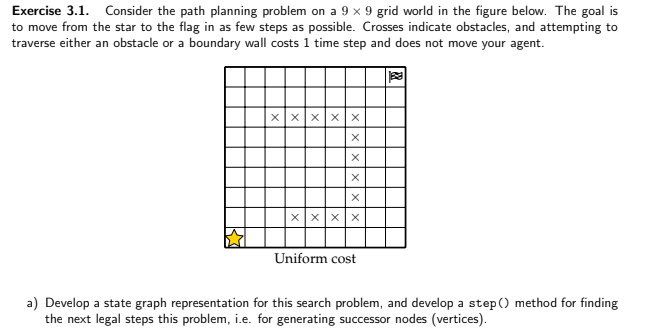
\includegraphics[scale=0.5]{31a.png}
\end{frame}

\begin{frame}{Tactics for approaching Exercises 3.1 and 3.2}
Try to map out what is required for designing (modelling) agent and environment interaction: \pause
\begin{itemize}
	\item What is the agent? \pause
	\item What is the environment? \pause
	\item What is the agents goal? \pause
	\item What are its costs? 
\end{itemize}
\end{frame}

\begin{frame}{Modules}
\pause
The \textbf{Environment Module} will model the world
\begin{itemize}
	\item Within the module, think about how you want to structure the interaction with the agent, and use this to define different classes.
\end{itemize}
\pause
\textbf{Search agent module} 
\begin{itemize}
	\item Recall the common ingredients of search agents
	\begin{itemize}
		\item Data structure (eg. queue, stack).
		\item goal state checker.
		\item A way to obtain neighbours of currently explored states.
	\end{itemize} \pause
	\item One way to approach this is to develop one module with an abstract search agent class that is reused for each concrete algorithm, another way you could seperate code for each algorithm.
\end{itemize}
\end{frame}

\begin{frame}{3.1 a}
Develop a state graph representation for this search problem, and develop a step() method for finding the next legal steps this problem, i.e. for generating successor nodes (vertices).\\
\begin{center} \pause

\includegraphics[scale=0.4]{envonly.png}
\end{center}
https://gist.github.com/aryaman-sh/e220d845ed0bb36f6335c49008dbcb1d
\end{frame}

\begin{frame}{3.1 }
b) Implement BFS for this problem (using a FIFO queue) using your step() function.
\\
\pause
c) Implement iterative-deepening DFS (IDDFS) for this problem using a length-limited LIFO queue, and reusing step().\\
\pause
\begin{center}

\includegraphics[scale=0.4]{31aqr.png}
\end{center}
https://gist.github.com/aryaman-sh/62d8da41f0963264149034b24cd504bb
\end{frame}

\begin{frame}{3.1 d}
Compare the performance of BFS and IDDFS in terms of
\begin{itemize}
	\item the number of nodes generated
	\item number of nodes on fringe when search terminates
	\item number of nodes on the expored set (if there is one) when the search terminates
	\item run time of the algorithm
\end{itemize}
\pause
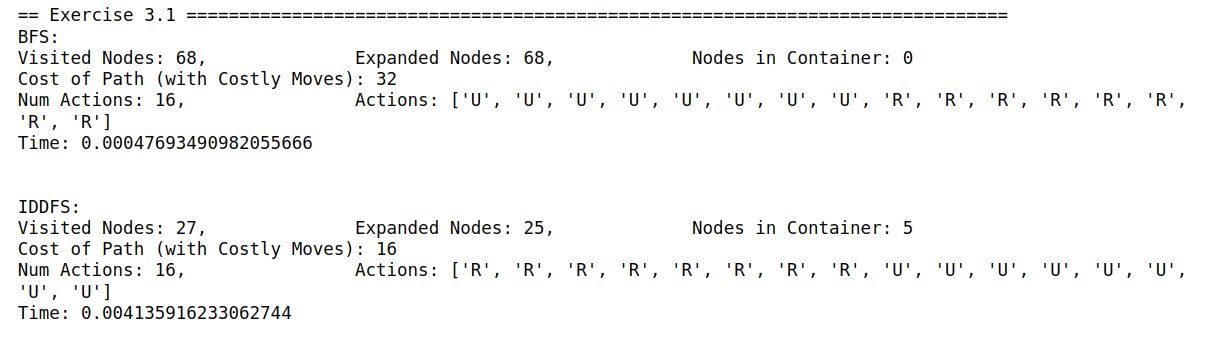
\includegraphics[scale=0.25]{31d.png}
\end{frame}

\begin{frame}{3.2}
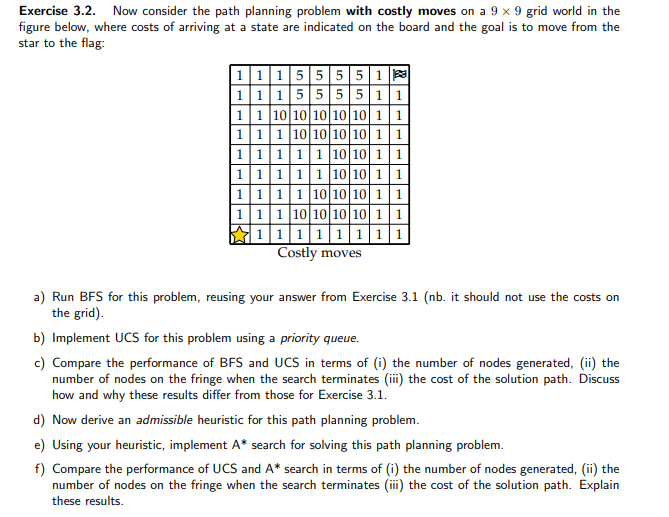
\includegraphics[scale=0.5]{32q.png}
\end{frame}

\begin{frame}{3.2 b}
Implement UCS for this problem using a priority queue.
\pause
\begin{itemize}
	\item consider heapq.heapify(container)
\end{itemize}
\pause
\begin{center}

\includegraphics[scale=0.4]{ucs.png}
\end{center}
https://gist.github.com/aryaman-sh/2c75adc2f425c0bac5c83817eb9b173f
\end{frame}

\begin{frame}{3.2 c}
Compare the performances of BFS and UCS in terms of 
\begin{itemize}
	\item the number of nodes generated
	\item the number of nodes on the fringe when the search terminated
	\item the cost of the solution path
\end{itemize}
Discuss how and why these results differ from those for 3.1\\
\pause
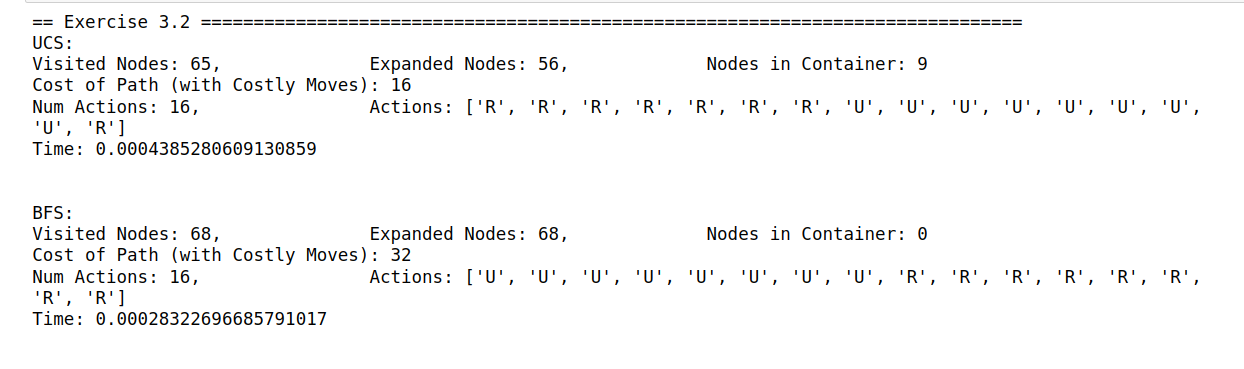
\includegraphics[scale=0.25]{32cans.png}
\end{frame}

\begin{frame}{3.2 d}
Now derive and \textbf{admissible} heuristic for this path planning problem.
\end{frame}

\begin{frame}{Informed search using heuristics}
Idea: Don't ignore the goal when selecting paths. \pause
\begin{itemize}
	\item Often there is extra knowledge that can be used to guide the search :\textbf{heuristics}. \pause
	\item h(n) is an estimate of the cost of the shortest path from node n to goal node. \pause
	\item h(n) needs to be efficient to compute. \pause
	\item h(n) does not overestimate, if there is no path from n to a goal with cost less than h(n). \pause
	\item An \textbf{admissible heuristic} is a nonnegative ($\geq 0$) heuristic function that never overestimates the actual cost of a path to a goal (it is optimistic)
\end{itemize}
\end{frame}

\begin{frame}{3.2 d}
Possible heuristic to use: \pause
\begin{itemize}
	\item Manhattan distance of each tile to its goal position \pause
\end{itemize}
Manhattan distance is admissible because every tile will have to be moved at least the number of spots in between itself and its correct position.
\end{frame}

\begin{frame}{Manhattan distance}
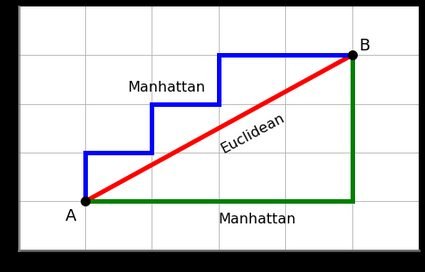
\includegraphics[scale=0.3]{manhattan_distance.jpeg}\\
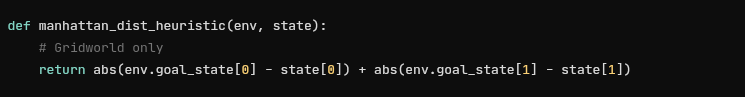
\includegraphics[scale=0.4]{32dcode.png}
\end{frame}

\begin{frame}{3.2 e}
Using your heuristic, implement $A^*$ search for solving this path problem. \pause
\begin{center}

\includegraphics[scale=0.4]{astarcode.png}
\end{center}
https://gist.github.com/aryaman-sh/c2ec9f4fde8e92b3f5a95f35a5298392
\end{frame}

\begin{frame}{3.2 f}
Compare the performances of UCS and $A^*$ search in terms of
\begin{itemize}
	\item the number of nodes generated
	\item the number of nodes on the fringe when the search terminates
	\item the cost of the solution path
\end{itemize}\pause
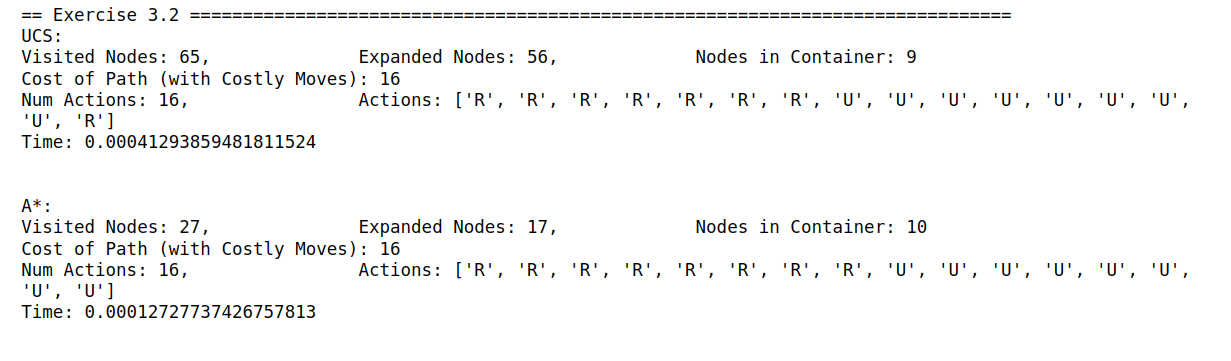
\includegraphics[scale=0.25]{32answer.png}
\end{frame}

\begin{frame}{3.3}
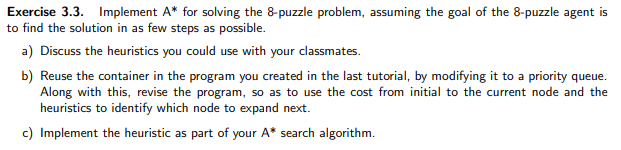
\includegraphics[scale=0.5]{33ques.png}
\end{frame}

\begin{frame}{3.3 a}
Possible heuristics to include: \pause
\begin{itemize}
	\item Hamming distance (i.e. number of tiles that are different between the current state and the goal state)\pause
	\item Manhattan distance of each tile to its goal position \pause
	\item the number of inversions\pause
\end{itemize}
All these heuristics would be admissible, but they may vary in how efficiently we can find the solution.
\end{frame}

\begin{frame}{3.3 b}
Reuse the container in the program you created in the last tutorial, by modifying it to a priority queue.
Along with this, revise the program, so as to use the cost from initial to the current node and the
heuristics to identify which node to expand next. \pause
\begin{center}

\includegraphics[scale=0.4]{33code.png}
\end{center}
https://gist.github.com/aryaman-sh/169224a843fdd4d2db58094439aaf293
\end{frame}

\begin{frame}{3.3 c}
Comparing performance\\

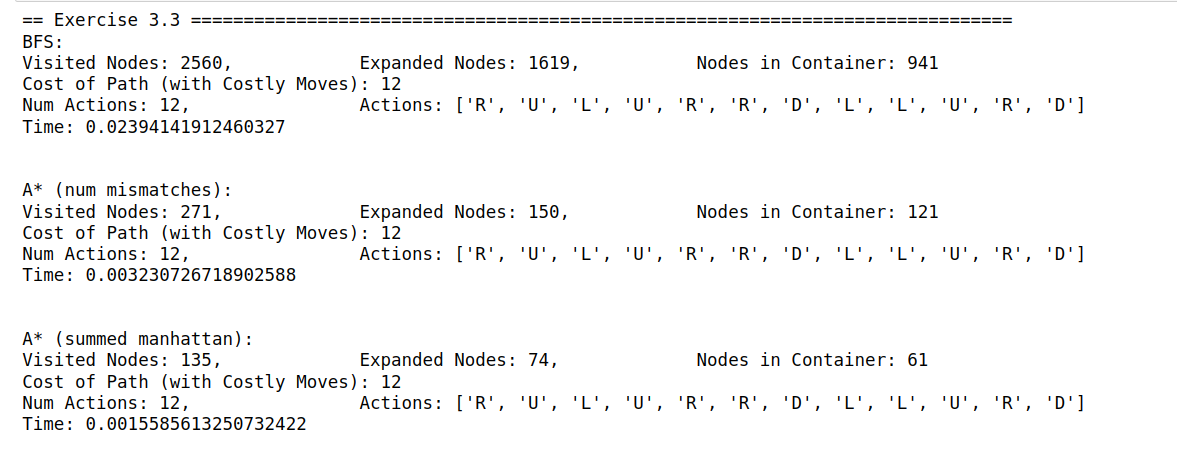
\includegraphics[scale=0.25]{33results.png}
\end{frame}

\begin{frame}{3.4}
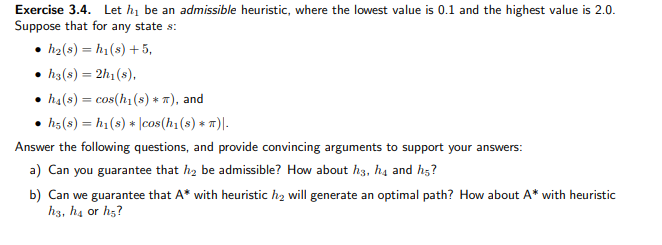
\includegraphics[scale=0.5]{34question.png}
\end{frame}

\begin{frame}{$h_2(s) = h_1(s)+5$}
\pause
We know that h1 is an admissible heuristic. That is to say, it does not overestimate the true cost to the goal.\\
$h_2(s) = h_1(s)+5$. 
\begin{itemize}
	\item We cant gurantee that $h_2(s)$ is asmissible because $h_2(s)$ is larger than $h_1(s)$. \pause
	\item We cannot say for sure whether or not $h_2(s)$ overestimates the true cost to the goal, and it is not admissible.
\end{itemize}
\end{frame}

\begin{frame}{$h_3(s) = 2h_1(s)$}
\pause
\begin{itemize}
	\item This heuristic will always be larger than $h_1(s)$. Thus for the same reason we cannot gurantee its admissibility.
\end{itemize}
\end{frame}

\begin{frame}{$h_4(s)=cos(h_1(s)* \pi)$}
\pause
\begin{itemize}
	\item We know $-1 \leq cos(x) \leq 1$ $\implies$ there may be some state s such that $cos(h_1(s)\pi)>h_1(s)$.
	\item $h_1(s)=0.1 \implies h_4(s)=0.99998>0.1$.
\end{itemize}
\end{frame}

\begin{frame}{$h_5(s)= h_1(s)*|cos(h_1(s)*\pi)|$}
\pause
\begin{itemize}
	\item Since $h_1(s)$ is being scaled by a values between 0 and 1. We can gurantee $h_5(s)\leq h_1(s)$.
	\item Since we know that $h_1(s)$ is admissible and thus never overestimates the true cost to the goal, we can gurantee the same for $h_5(s)$.
\end{itemize}
\end{frame}

\begin{frame}{3.4 b: Optimality}
\begin{itemize}
	\item We can gurantee $h_2$ generates optimal path. Why?\pause
	\item When choosing between two possible nodes to expand in $A^*$, the priority queue used $f(s)= g(s) + h(s)$. \pause
	\item Whichever node has lowest f value will be chosen next. \pause 
	\item Thus if $h_1(s)$ is admissible heuristic (will lead to optimal solution), replacing with $h_1(s)+5$ will never change the order of queued nodes.
\end{itemize}
\end{frame}

\begin{frame}{Optimality $h_3(s)$}
$h_3(s) = 2h_1(s)$
\pause
\begin{itemize}
	\item A similar argument cannot be used for $h_3$\pause
	\item The shift here is not constant but multiplicative.
\end{itemize}
\end{frame}

\begin{frame}{Optimality $h_4(s)$, $h_5(s)$}
\pause
$h_4(S) = cos(h_1(s)\pi)$
\begin{itemize}
	\item The values can change fairly drastically, and this heuristic is no longer admissible.
\end{itemize}
\pause
$h_5(s)= h_1(s)(cos(h_1(s)\pi)$\pause
\begin{itemize}
	\item $h_5$ is always equal to or less than $h_1$. $h_1$ is being scaled down by a number that is always positive and $\leq 1$. \\
	\item $\implies h_5$ is admissible and will generate an optimal solution. 
\end{itemize}
\end{frame}
\end{document}